\chapter{Introduction}
Internet Information Retrieval (IIR) is a research domain in computer science concerned with the retrieval, extraction, classification, and presentation of information from the Internet. The toolkit provides functionality which is often needed to perform IIR tasks such as crawling, classification, and extraction of various types of information.

\section{What Palladian is}
%TODO contributions
Palladian is a collection of algorithms for text processing focused on \textbf{ classification}, \textbf{ extraction}, and \textbf{ retrieval}. The concept of Palladian is system to reuse algorithms that are freely available and build upon them to drive research. When trying to learn and advance in a new field of research, one has to play around with many code snippets from various authors, this toolkit tries to ease this process by making external libraries accessible through a single interface. This way new algorithms can be quickly compared to the state-of-the-art.
The best results from students at the Dresden University of Technology find their way into the toolkit allowing other users to create more advanced programs in the future.

Our main contributions to the research community are:
\begin{enumerate}
\item New algorithms in the fields of classification and extraction that can easily be tested and applied to other projects.
\item Single interface access to bundles of well established algorithms.
\item Helping make research more transparent by fomenting users to reproduce results with the included algorithms.
\end{enumerate}

Figure \ref{fig:architecture} shows the main packages of Palladian. The focus is evidently on retrieval (Crawler, API access, feed reading...), preprocessing (tokenization, sentence splitting...), classification (KNN, Dictionary Classifier...), and extraction (named entities, tags...).

\begin{figure}[ht!]
\centering
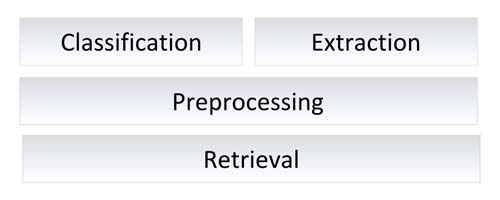
\includegraphics[width=0.6\textwidth]{img/architecture.pdf}
\caption{Important Packages of Palladian.}
\label{fig:architecture}
\end{figure}

\section{What Palladian is NOT}
Palladian is not a full natural language processing suite nor does it contain a \textit{ full} set of algorithms in the fields of classification, extraction, and information retrieval. Palladian is not a commercial product either, we like to answer questions as soon and comprehensive as possible but cannot guarantee this support.

\section{Who the Intended User is}
In general everybody is welcome to use Palladian, but the researchers that would develop algorithms and would like to quickly test or compare them are the focus. Researchers likely to help other researchers, that won't mind a software that is not perfect, bug-free or commercial.

\section{License}
The complete source code is licensed under the Apache License 2.0. All source files should include the following license snippet at the very top.

\begin{verbatim}
Copyright 2010 David Urbansky, Klemens Muthmann
Licensed under the Apache License, Version 2.0 (the "License"); you may not
use this file except in compliance with the License. You may obtain a copy of
the License at

http://www.apache.org/licenses/LICENSE-2.0

Unless required by applicable law or agreed to in writing, software
distributed under the License is distributed on an "AS IS" BASIS, WITHOUT
WARRANTIES OR CONDITIONS OF ANY KIND, either express or implied.
See the License for the specific language governing permissions and
limitations under the License.
\end{verbatim}

\section{Evaluation Measures for IIR Systems}

This sections outlines important evaluation measures which are typically used for comparing and scoring algorithms and techniques in (Internet) Information Retrieval. Our goal is to give just a brief overview, more details can be found in the referenced literature.

% TODO ... work for the holidays

\subsection{Precision, Recall, and F-measure} \label{sec:Introduction:PrRcF1}

Considering a specific query (e.\,g. \textit{apples OR oranges}), a set of relevant and non-relevant documents and a subset of retrieved -- i.\,e. found -- documents, we can distinguish between four disjoint sets, which can be classified as combinations of the attributes ``true'' or ``false'' with ``positive'' or ``negative'', as depicted in Figure~\ref{fig:PrecisionRecall}. Documents which have been filtered out by the system errnously are classified as ``false negatives'', irrelevant documents which are presented to the user are classified as ``false positives''. Precision $P$ and Recall $R$ can be determined as stated in Equations~\ref{eqn:Precision} and \ref{eqn:Recall}. Intuitively, both take a range between 0 and 1 inclusively, where 1 denotes the optimum.

\begin{equation}
	\label{eqn:Precision}
	Precision = P = \frac{\left|\,\mathit{relevant, retrieved docs}\,\right|}{\left|\,\mathit{retrieved docs}\,\right|} = \frac{\left|\,\mathit{true positives}\,\right|}{\left|\,\mathit{true positives}\,\right| + \left|\,\mathit{false positives}\,\right|}
\end{equation}

\begin{equation}	
	\label{eqn:Recall}
	Recall = R = \frac{\left|\,\mathit{relevant, retrieved docs}\,\right|}{\left|\,\mathit{relevant docs}\,\right|} = \frac{\left|\,\mathit{true positives}\,\right|}{\left|\,\mathit{true positives}\,\right| + \left|\,\mathit{false negatives}\,\right|}
\end{equation}

The F-measure combines both the Precsion and the Recall to one value. Usually the so called $F_1$ score is calculated by employing a harmonic mean as depicted in Equation~\ref{eqn:F1Measure}. The universal F-measure which allows weighting, and thus prioritizing, Precision and Recall values differently is described in \cite[p.\,156]{Manning:2009}. 

\begin{equation}
	\label{eqn:F1Measure}
	F_1 = \frac{2 \cdot P \cdot R}{P + R}
\end{equation}


\begin{figure}[t!]
\label{fig:PrecisionRecall}
\centering
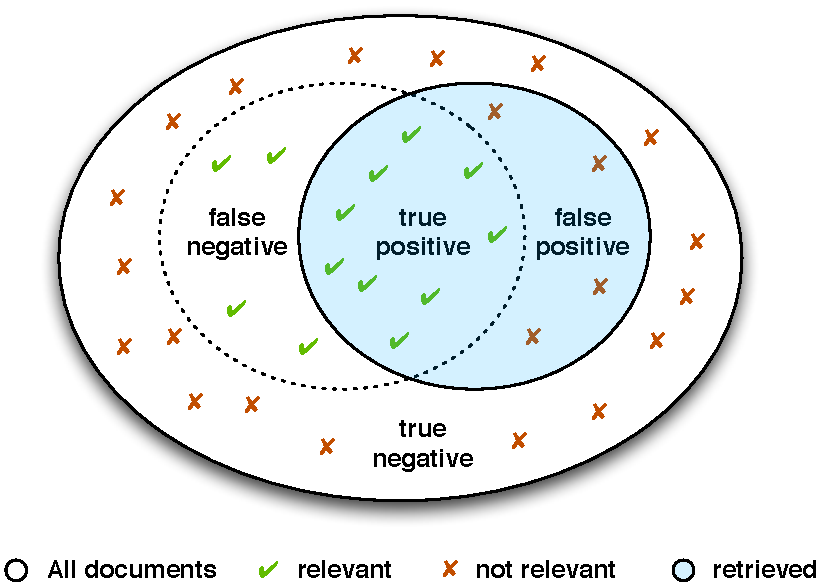
\includegraphics[width=0.6\textwidth]{img/PrecisionRecallSets.pdf}
\caption{Set of Documents as Basis for Precision and Recall \cite{katz2010diploma}.}
\end{figure}

\subsection{Mean Squared Error, Root Mean Squared Error}

The Mean Squared Error (MSE) is used for measuring the deviation of estimated or predicted numeric values from their actual values. Therefor, the average of the quadratic differences between each actual value $y$ and the predicted value $\bar y$ is calculated. By squaring down the differences, the bigger errors are weighted stronger compared to small errors. The Root Mean Squared Error (RMSE) additionally extracts the square root from the MSE, as depicted in Equation~\ref{eqn:RMSE}.

\begin{equation}
	\label{eqn:RMSE}
	\mathit{RMSE} = \sqrt{\frac{1}{n} \sum\limits_{i=1}^{n}(y_i - \bar y_i)^2}
\end{equation}

\subsection{Precision at k, Average Precision, Mean Average Precision}

Precision, Recall and F-measure as described in Section~\ref{sec:Introduction:PrRcF1} are metrics, which only consider unsorted sets of items. To evaluate ordered lists, which are ranked by relevance for example, the following measures can be employed.

``Precision at k'' denotes the precision for a ranked sublist of the first k documents as illustrated in Equation~\ref{eqn:PrAtK}. The binary function $rel(i)$ takes a value of 1, if the document at position $i$ is relevant for the current query, 0 elsewise \cite{Mahesh:1999}. For example, $P(k = 10)$ with 5 relevant and 5 irrelevant documents results in a value of 0.5.

\begin{equation}
	\label{eqn:PrAtK}
	P(k) = \frac{\sum_{i = 1}^{k} \mathit{rel}(i)}{k}
\end{equation}

Equation~\ref{eqn:AP} shows the Average Precision (AP), which is the sum of the precisions from Equation~\ref{eqn:PrAtK} where $rel(i)$ equals a value of 1, divided by the total count of relevant documents in the sublist of $n$ results \cite{Mahesh:1999}. Table~\ref{tab:ExampleMAP} gives a calculation example.

\begin{equation}
	\label{eqn:AP}
	\mathit{AP} = \frac{\sum_{k = 1}^{n} P(k) \mathit{rel}(k)}{R}
\end{equation}

% Daten siehe --> AveragePrecision.numbers
\begin{table}[h!tbp]
	\label{tab:ExampleMAP}
	\centering
	\begin{tabular}{|c|c|c|c|c|}
				
		\hline
		Rank k & relevant? & \# relevant & P(k) & AP  \\
		\hline
				
		1  & $\checkmark$ & 1 & 1                                & 1   \\ \hline
		2  &              & 1 & $1/2 = 0.5$         & 1   \\ \hline
		3  & $\checkmark$ & 2 & $2/3 \approx 0.67$  & $(1 + 2/3) / 2 \approx 0.83$  \\ \hline
		4  & $\checkmark$ & 3 & $3/4 = 0.75$        & $(1 + 2/3 + 3/4) / 3 \approx 0.81 $    \\ \hline
		5  & $\checkmark$ & 4 & $4/5 = 0.8$         & $(1 + 2/3 + 3/4 + 4/5) / 4 \approx 0.80$    \\ \hline
		6  & $\checkmark$ & 5 & $5/6 \approx 0.83$  & $(1 + 2/3 + 3/4 + 4/5 + 5/6) / 5 \approx 0.81$    \\ \hline
		7  &              & 5 & $5/7 \approx 0.71$  & $(1 + 2/3 + 3/4 + 4/5 + 5/6) / 5 \approx 0.81$    \\
		
		 \hline
	\end{tabular}

	\caption{Example for calculating Precision and Average Precision for a ranked list.}
\end{table}

% TODO ... MAP


\subsection{Mean Reciprocal Rank}

\section{Alternative and Complimentary Toolkits}

\label{sec:alternativesToPalladian}
Some functionalities of this toolkit are covered in other libraries. If you can't find the functionality you need in Palladian you might want to take a look at these alternatives. Some of the objectives of Palladian are to create new functionalities or improve existing ones, not to reinvent the wheel and redo work that functions well in other libraries.

%TODO clean up list, bullets or table of services
\begin{enumerate}

	\item \textbf{AlchemyAPI} \cite{alchemyapi} is a commercial web-service that can be used via several programming languages. The service offers named entity recognition, text classification, language identification, concept tagging, keyword extraction, content scraping, and web page cleaning.
The service comes in 4 variants: free, basic, professional, and metered.

	\item \textbf{Apache Mahout} \cite{settings2apache} is a Java-based machine learning library. Its main features are collaborative filtering, user and item based recommenders, (fuzzy k-means clustering, mean shift clustering, latent dirichlet process allocation, singular value decomposition, parallel frequent pattern mining, complementary naive bayes classifier, and a random forest decision tree based classifier.
The library is licensed under the Apache Software license.

	\item \textbf{Balie} \cite{balie} is a Java-based information extraction library. Its main features are language identification, tokenization, sentence boundary detection, and named entity recognition (using dictionaries).
The library is licensed under the GNU GPL and supports English, German, French, Romanian, and Spanish as input languages.

	\item \textbf{Classifier4J} \cite{classifier4j} is a very simple Java library for text classification. Besides Bayesian and vector classification, it offers a text summary feature.
	
	\item \textbf{ClearTK} \cite{cleartk, ogren_cleartk:uima_2008} is a Java-based toolkit for developing statistical natural language processing components. It is based on the Apache UIMA framework for text analysis. It provides a wrapper interface for various components and libraries. ClearTK per se is available under a BSD license, whereas some of the wrapped components are licensed under a GPL license.

	\item \textbf{ContentAnalyst} \cite{contentanalyst} is a commercial platform for text analytics. The platform's main features are concept search, dynamic clustering, near-duplicate document identification, automatic summarization, text classification, and latent semantic indexing.

	\item The \textbf{Dragon Toolkit} \cite{zhou2007dragon} is a Java-based development package for information retrieval and text mining. Its main features are text classification, text clustering, text summarization, and topic modeling.

	\item \textbf{FreeLing} \cite{atserias2006freeling} is a natural language processing library written in C++. Its main features are Text tokenization, sentence splitting, morphological analysis, sSuffix treatment, retokenization of clitic pronouns, flexible multiword recognition, contraction splitting, probabilistic prediction of unkown word categories, named entity detection, recognition of dates, numbers, ratios, currency, and physical magnitudes, PoS tagging, chart-based shallow parsing, named entity classification,  WordNet based sense annotation and disambiguation, Rule-based dependency parsing, and nominal correference resolution.
It is licensed under GPL and supports Spanish, Catalan, Galician, Italian, English, Welsh, Portuguese, and Asturian as languages. An online demo is available under \url{http://garraf.epsevg.upc.es/freeling/demo.php}.

	\item \textbf{GATE} \cite{cunningham2002gate} is a Java-based text mining and processing framework. The framework itself comes with few text processing features but many plugins can be used and chained into a text engineering pipeline.
The framework is licensed under the GNU Lesser General Public License.

	\item The \textbf{Illinois Cognitive Computation Group} \cite{illinoisccg} has a list of ready to use programs for semantic role labeling, text chunking, named entity tagging, named entity discovery, PoS tagging, unsupervised rank aggregation, and named entity similarity metrics.
	
	\item \textbf{JTMT} (Java Text Mining Toolkit) \cite{JTMT} is an assorted collection of Java code for various text mining and information retrieval tasks. Different components are explained in-depth in the author's blog. The toolkit is licensed under the Lesser GNU General Public License (LGPL).
	
	\item \textbf{jtokenizer} \cite{jtokenizer} is a Java-based library providing a multitude of different tokenizer implementations. It also offers a GUI frontend for experimenting with the different tokenizers. The library is licensed under GNU Lesser GPL.

	\item \textbf{Julie NLP} \cite{tomanek2007uima,hahn2008overview} is a Java-based toolkit of UIMA based text processing components. The toolkit can be used for semantic search, information extraction, named entity recognition, and text mining.
The Toolkit is licensed under the Common Public License.

	\item \textbf{Language Computer} \cite{lanuagecomputer} provides commercial products for sentence splitting, tokenization, PoS tagging, named entity recognition, co-reference resolution, attribute extraction, relationship extraction, event extraction, question answering, and text summarization.

	\item \textbf{Lemur Project} \cite{lemur} provides a toolkit with search engines and tools for research tasks in information retrieval and text mining. The project was founded in 2000 by the Center for Intelligent Information Retrieval (CIIR) at the University of Massachusetts, Amherst. Updates for the toolkit are released on a regular basis. The toolkit is written in C++, but also offers C\# and Java APIs. Beside the Lemur toolkit itself, the project offers a search engine called ``Indri'' and a browser plugin to capture users' query and browsing behaviours.

	\item \textbf{Lingo3G} \cite{lingo3g} is a text clustering engine that organizes text collections into hierarchical clusters.
The software is commercial but \cite{stefanowski2003carrot} offers an open source alternative for text clustering algorithms written in Java. The algorithms integrate with other programming or scripting languages such as PHP, Ruby, and C\# too.

	\item \textbf{LingPipe} \cite{lingpipe} is a text processing toolkit using computational linguistics. LingPipe is written in Java. Its main features are topic classification, named entity recognition, clustering, PoS tagging, sentence detection, spelling correction, database text mining, string comparisons, interesting phrase detection, character language modeling, chinese word segmentation, hyphenation and syllabification, sentiment analysis, language identification, singular value decomposition, logistic regression, expectation maximization, and word sense disambiguation.
LingPipe is available under a free license for academic use and several commercial licenses.

	\item \textbf{Mallet} \cite{mccallum2002mallet} is a Java-based toolkit for statistical natural language processing. Its main features are text classification, sequence tagging (PoS tagging), topic modeling, and numerical optimization.
The toolkit is licensed under the Common Public License.

	\item \textbf{Mate Tools} \cite{mateTools} is a library for lemmatization, part-of-speech tagging, dependency parsing, and semantic role labeling. It is licensed under GNU GPL v2 license.

	\item \textbf{MinorThird} \cite{cohen2004minorthird} is a Java-based toolkit for text processing. Its main features are annotating text, named entity recognition, and text classification.
The toolkit is licensed under the BSD license.

	\item \textbf{MontyLingua} \cite{liu2004montylingua} is a Python and Java-based toolkit for natural language processing (English only). Its main features are tokenization, PoS tagging, lemmatization, and natural language summarization.
The toolkit is free for non-commercial use and licensed under the MontyLingua version 2.0 License.

	\item \textbf{MorphAdorner} \cite{morphadorner} is a Java-based command line program for text processing. Its main features are language recognition, lemmatization, name recognition, PoS tagging, noun pluralization, sentence splitting, spelling standardization, text segmentation, verb conjugation, and word tokenization.
The program is licensed under a NCSA style license.

	\item \textbf{NaCTeM Software Tools} \cite{nactem} are programs for natural language processing and text mining that are made available by the National Centre for Text Mining. The programs include functionality for PoS tagging, syntactic parsing, named entity recognition, sentence splitting, text classification, and sentiment analysis.

	\item \textbf{NLTK} \cite{loper2002nltk} is a Python-based natural language processing toolkit. Its main features are tokenization, stemming, PoS tagging, text classification, and syntactic parsing.
The toolkit is licensed under the Apache 2.0 license.

	\item \textbf{OpenCalais} \cite{opencalais} is a web service that performs named entity recognition, fact and event extraction.
The web service is free for commercial and non-commercial use but limited to 50,000 transactions a day. A professional plan is available too including more transactions and an service license agreement.

	\item \textbf{OpenNLP} \cite{opennlp} is a toolkit of various open source natural language processing packages. The goal of this toolkit is to integrate several stand-alone projects to increase the interoperability. Algorithms in this toolkit include but are not limited to tokenization and named entity recognition.

	\item The \textbf{RASP System} \cite{briscoe2006second} is a C and Lisp-based toolkit for natural language processing (English only). Its main features are tokenization, PoS tagging, lemmatization, morphological analysis, and grammar-based parsing.
The toolkit is free for non-commercial use and licensed under the RASP System License.

	\item The \textbf{Rosette Linguistic Platform} \cite{rosette} is a software suite that can perform name translation, name matching, named entity recognition, morphological analysis, and language identification. The suite works for 55 European, Asian, and Arabic languages.
The software is a commercial product.

	\item \textbf{The Semantic Discovery Toolkit} \cite{semanticdiscovery} is a set of tools under active development focussing on NLP, machine learning, XML parsing, crawling, parallel processing. It further provides wrapper classes for several related implementations. The toolkit is under GNU LGPL.

	\item \textbf{Stanford NLP} \cite{stanfordnlp} is a set of Java-based natural language processing libraries. Their main features are PoS tagging, named entity recognition, Chinese word segmentation, and classification.
The software distributions are licensed under the GNU Public License.

	\item \textbf{SRILM -- The SRI Language Modeling Toolkit} \cite{stolcke2002srilm} is a C++-based toolkit for language modeling. Its main features are speech recognition, statistical tagging and segmentation, and machine translation.
The toolkit is free for non-commercial use and licensed under the SRILM Research Community License.

	\item \textbf{TextAnalyst} \cite{textanalyst} is a commercial text processing software offering text summarization, semantic information retrieval, meaning extraction, and text clustering.

	\item \textbf{VisualText} \cite{visualtext} is a natural language processing software that addresses named entity recognition, text indexing, text filtering, text classification, text grading, and text summarization.

	\item \textbf{Watchmaker Framework} ``is an extensible, high-performance, object-oriented framework for implementing platform-independent evolutionary/genetic algorithms in Java. The framework provides type-safe evolution for arbitrary types via a non-invasive API.'' \cite{watchmaker}. Watchmaker is Open Source Software under an Apache license.

	\item \textbf{Weka} \cite{hall2009weka} is a Java-based machine learning and data mining library. The library contains a large set of machine learning algorithms such as Support Vector Machines, Neural Networks, Naive Bayes, k-nearest neighbor for but not limited to (text) clustering, (text) classification, and regression.
The library is licensed under the GNU General Public License.

\end{enumerate}
